\subsection{Szegélyek}

%37
\begin{frame}
  A szegélyeknek állítható a
  \begin{itemize}
    \item stílusa (\texttt{border-style}),
    \item szélessége (\texttt{border-width}), és a 
    \item színe (\texttt{border-color}).
  \end{itemize}
  Megjegyzések:
  \begin{itemize}
    \item Utóbbi kettő csak a stílus beállítása esetén működik.
    \item Minden paraméter állítható külön az egyes oldalakra is.
  \end{itemize}
\end{frame}

%38
\begin{frame}
  \begin{exampleblock}{\textattachfile{szegelyek1.html}{szegelyek1.html}}
    \scriptsize
    \lstinputlisting[style=HTML,linerange={14-17},numbers=left,firstnumber=14]{szegelyek1.html}
  \end{exampleblock}
  \begin{columns}[T]
    \column{0.25\textwidth}
      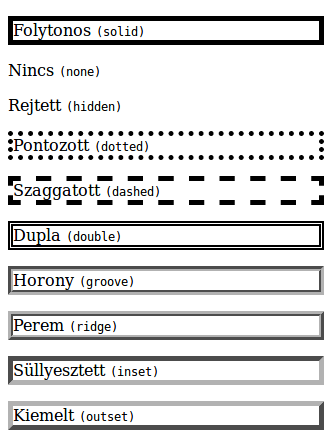
\includegraphics[scale=0.25]{szegelyek1.png}
    \column{0.7\textwidth}
      Oldalankénti szegélystílusok megadhatók:
      \begin{itemize}
        \item 1-4 érték megadásával, pl. \\ \texttt{border-style: dotted dashed solid none;}
        \item Oldalakra vonatkozó tulajdonságokkal: 
        \texttt{border-*-style}, ahol \texttt{*} helyén állhat 
        \texttt{top}, \texttt{right}, \texttt{bottom}, \texttt{left}.
      \end{itemize}
  \end{columns} 
\end{frame}

%39
\begin{frame}
  \begin{columns}[c]
    \column{0.6\textwidth}
      Ha a \texttt{boder-style}-nak
      \begin{description}[m]
        \item[1 értéke van] \hfill \\ \texttt{felül-jobb-alul-bal} (minden 
        oldalra ugyanazt a stílust állítja)
        \item[2 értéke van] \hfill \\ \texttt{felül-alul jobb-bal}
        \item[3 értéke van] \hfill \\ \texttt{felül jobb-bal alul}
        \item[4 értéke van] \hfill \\ \texttt{felül jobb alul bal} (óramutató 
        járása szerint)
      \end{description}
      \vfill
      Hasonlóképpen lehet oldalanként szabályozni a margókat és 
      kitöltéseket is.
    \column{0.35\textwidth}
      \begin{center}
        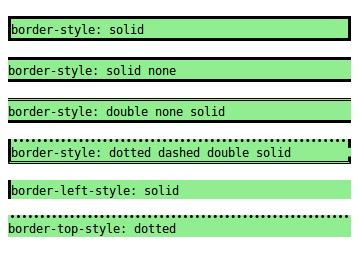
\includegraphics[width=\textwidth]{szegelyek2.png} \\
        \textattachfile{szegelyek2.html}{szegelyek2.html}
      \end{center}
  \end{columns} 
\end{frame}

%40
\begin{frame}
  \begin{columns}[c]
    \column{0.5\textwidth}
      Ha táblázatok szomszédos cellái közös, de eltérő stílusú szegélyeket 
      használnak, akkor
      \begin{description}[m]
        \item[\texttt{none}] \hfill \\ 
          ha a szomszédnak be van állítva a szegélye, az fog megjelenni
        \item[\texttt{hidden}] \hfill \\ 
          még ha be is van állítva a szomszéd szegélye, akkor sem 
          fog megjelenni
      \end{description}
    \column{0.5\textwidth}
      \begin{center}
        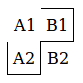
\includegraphics[scale=0.5]{szegelyek3.png}
      \end{center}
      \begin{exampleblock}{\textattachfile{szegelyek3.html}{szegelyek3.html}}
        \scriptsize
        \lstinputlisting[style=HTML,linerange={21-21},numbers=left,firstnumber=21]{szegelyek3.html}
        \lstinputlisting[style=HTML,linerange={26-26},numbers=left,firstnumber=26]{szegelyek3.html}
      \end{exampleblock}
  \end{columns} 
\end{frame}

%41
\begin{frame}
  Rövidítések
  \begin{description}[m]
    \item[\texttt{border: width style color}] \hfill \\ 
      Minden oldalon beállítja a szegély szélességét, stílusát, színét.
    \item[\texttt{border-*: width style color}] \hfill \\ 
      A \texttt{*} lehet \texttt{top}, \texttt{right}, \texttt{bottom} 
      és \texttt{left}; csak ezekre állítja a fenti három tulajdonságot.
  \end{description}
\end{frame}
